\documentclass[12pt, letterpaper]{article}

\usepackage[polish]{babel}
\usepackage{graphicx}
\usepackage{fontspec}
\usepackage{lilyglyphs}

\graphicspath{{./img/}}

\title{Sprawozdanie}
\author{
    Kamil Niżnik 145238 \\
    Jakub Kwiatkowski 145356
}
\date{Grudzień 2021}


\begin{document}

\newlength{\imagewidth}
\setlength{\imagewidth}{0.8\textwidth}

\maketitle

\part*{Omówienie}

\section{Temat}

Celem projektu było zaimplementowanie prostego systemu OMR
(ang. Optical Music Recognition System) wykrywającego podstawowe
symbole stosowane w zapisie nutowym:
\begin{itemize}
    \item Klucze
          \begin{itemize}
              \item wiolinowy (\textit{G-clef}) - \clefG
              \item basowy (\textit{F-clef}) - \clefF
          \end{itemize}

    \item Nuty
          \begin{itemize}
              \item całą nutę (\textit{semibreve}) - \semibreve
              \item półnutę (\textit{minim}) - \minim
              \item ćwierćnutę (\textit{crotchet}) - \crotchet
              \item ósemkę (\textit{quaver}) - \quaver
          \end{itemize}
\end{itemize}

System został zaimplementowany z myślą o odręcznie pisanych nutach,
dlatego może, lecz nie musi, działać z nutami drukowanymi.


\section{Opis działania}

System został zaprojektowany w sposób umożliwiający potokowe przetwarzanie obrazu.


System można podzielić na trzy części:
\begin{itemize}
    \item Preprocessing \ref{sec:preprocessing}
    \item Object detection \ref{sec:detection}
    \item Object recognition \ref{sec:recognition}
\end{itemize}

\subsection{Preprocessing}
\label{sec:preprocessing}

Ze względu na charakter danych wejściowych, tj. zdjęć wykonanych aparatem smartfonu,
niezbędny jest etap, który ma za zadanie oddzielić tło od elementów pierwszoplanowych,
usunąć szum czy obrócić obraz do prawidłowej pozycji.
Etap ten został rozbity na pięć zadań:

\begin{enumerate}
    \item Desaturacja \ref{subsec:desaturation}
    \item Binaryzacja i odszumianie \ref{subsec:binarization}
    \item Prostowanie \ref{subsec:rotation}
    \item Wykrywanie linii \ref{subsec:line-detection}
    \item Usuwanie pięciolinii \ref{subsec:staff-removal}
\end{enumerate}

\begin{figure}
    \centering
    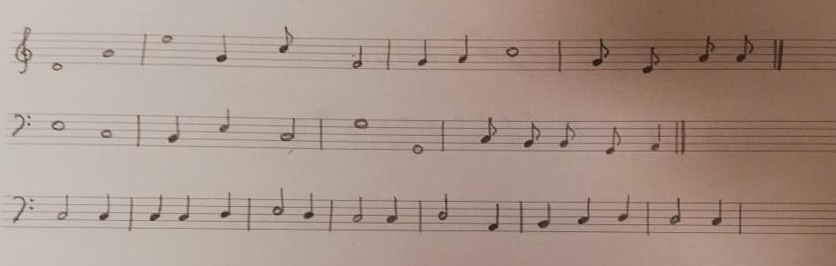
\includegraphics[width = \imagewidth]{0_source}
    \caption[Source]{Obraz oryginalny}
    \label{img:source}
\end{figure}

\subsubsection{Desaturacja (\textit{\small grayscaling})}
\label{subsec:desaturation}

\textit{Pierwszy krok przetwarzania, \textbf{\small niezbędny} do zastosowania pozostałych technik.}
\\
\\
Desaturacja usuwa z obrazu informację o kolorze.
W przypadku rozpoznawania nut informacja o kolorze jest zbędna,
ponieważ standardowy zapis muzyczny używa jedynie czarnych znaków.
\\
\\
Efekt desaturacji rysunku \ref{img:source} został przedstawiony na
rysunku \ref{img:desaturated}

\begin{figure}
    \centering
    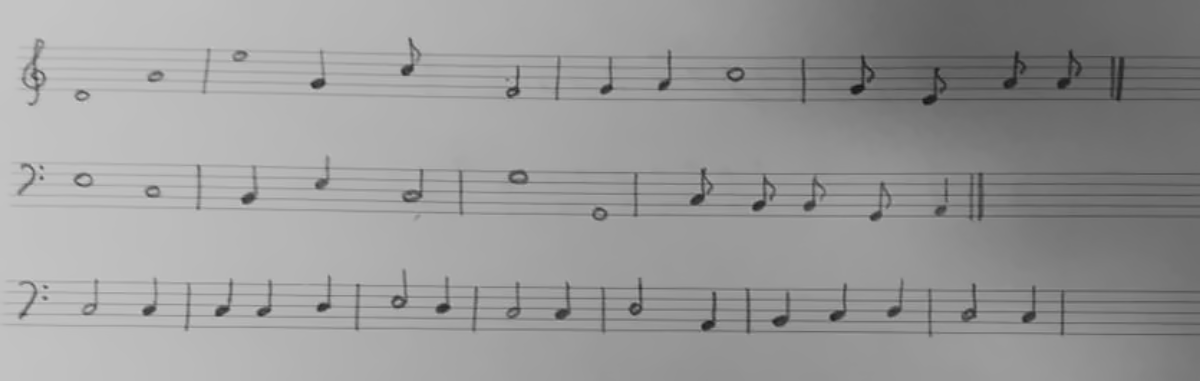
\includegraphics[width=\imagewidth]{1_desaturated}
    \caption[Desaturated]{Obraz skonwertowany do skali szarości}
    \label{img:desaturated}
\end{figure}

\subsubsection{Odszumianie i binaryzacja (\textit{\small denoising \& thresholding})}
\label{subsec:binarization}

Binaryzacja kompresuje obraz do dwóch kolorów: czarnego i białego.
Upraszcza ona oddzielenie obiektów pierwszoplanowych od tła dzięki zwiększeniu kontrastu
między obiektami.
\\
\\
Ze względu na niejednorodne oświetlenie i inne przeszkody utrudniające
klasyczną binaryzację w programie zastosowano algorytm
\emph{local adaptive thresholding}, który dobiera wartość progu bazując na
jasnościach sąsiadujących pikseli.
\\
\\
Odszumianie służy usunięciu niewielkich, losowych skupisk pikseli
wynikających z niedoskonałości zdjęcia i zakłócających zbinaryzowany obraz.
\\
\\
Efekty binaryzacji i odszumiania rysunku \ref{img:desaturated} zostały przedstawione na
rysunku \ref{img:desaturated}

\begin{figure}
    \centering
    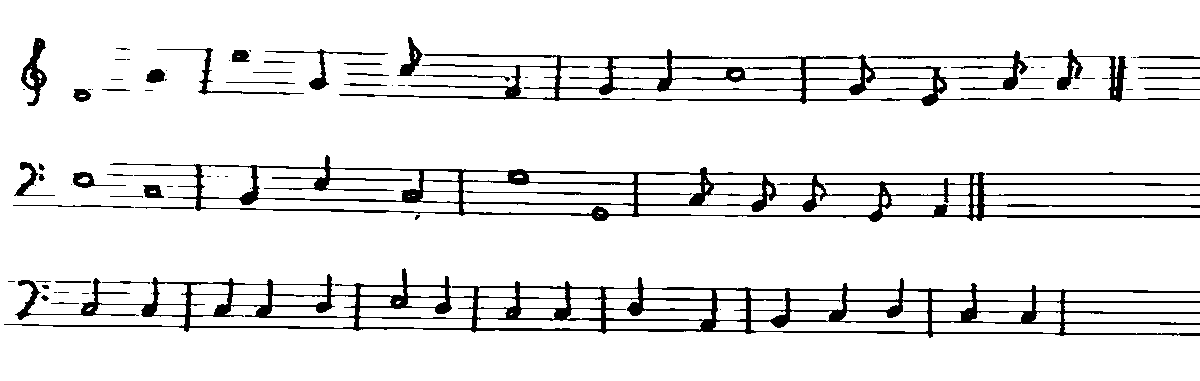
\includegraphics[width = \imagewidth]{2_binarized}
    \caption[Binarized]{Zbinaryzowany i odszumiony obraz \ref{img:desaturated}}
    \label{img:binarized}
\end{figure}

\subsubsection{Prostowanie}
\label{subsec:rotation}

Prostowanie ma na celu obrócenie obrazu tak, aby linie pięciolinii
były w położeniu horyzontalnym.

W implementacji wypróbowaliśmy dwie techniki znajdowania kąta obrotu:

Pierwszą metodą jest \textit{Projection Profile} -
kąt obrotu wyliczany jest na podstawie różnicy maksimów
histogramów generowanych co pewien mały kąt.
\\
\\
Druga metoda natomiast wykorzystuje transformatę Hougha
do znalezienia pięciolinii i na podstawie znalezionych
kątów wylicza kąt obrotu.
\\
\\
Efekty prostowania rysunku \ref{img:desaturated} zostały przedstawione na
rysunku \ref{img:desaturated}

\begin{figure}
    \centering
    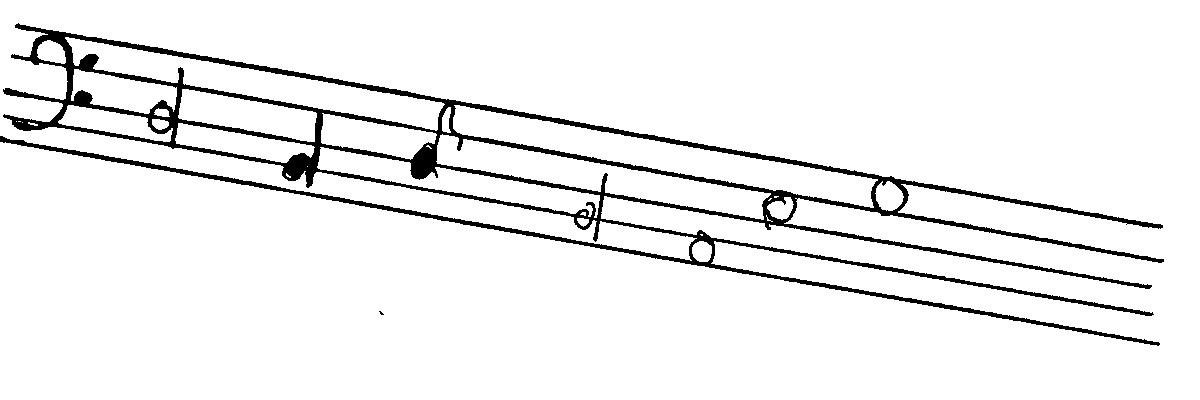
\includegraphics[width = \imagewidth]{3.1_binarized}
    \caption[Rotated]{Oryginalny obraz}
    \label{img:rotated}
    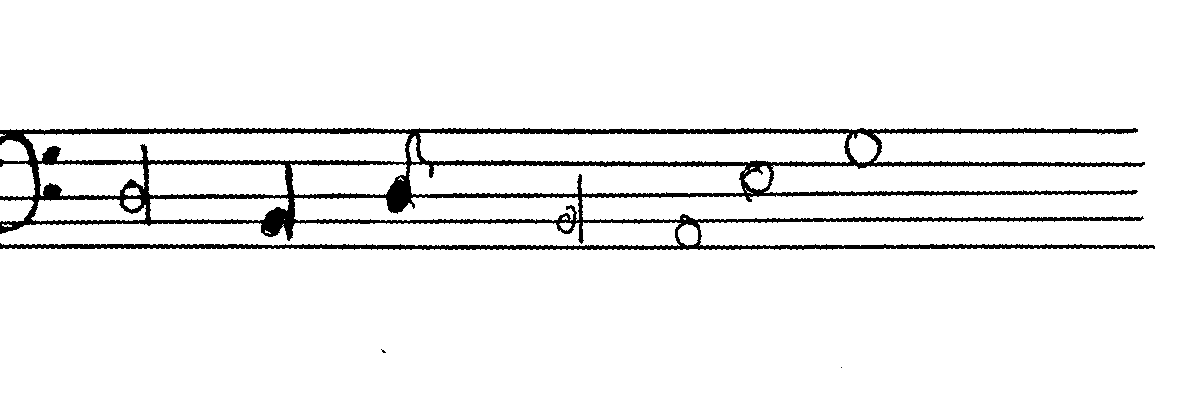
\includegraphics[width = \imagewidth]{3.2_straightened}
    \caption[Straightened]{Obraz obrócony do pozycji horyzontalnej}
    \label{img:straightened}
\end{figure}

\subsubsection{Wykrywanie linii}
\label{subsec:line-detection}
Po wstępnym przetworzeniu zdjęcia dokonywana jest detekcja,
a następnie usunięcie pięciolinii ze zdjęcia.
Może to być osiągnięte na wiele sposobów,
a dobór odpowiedniej techniki wciąż jest przedmiotem opracowań naukowych.
\\
\\
W niniejszej implementacji do wykrywania linii wykorzystano operację
morfologiczną otwarcia z elementem strukturalnym
odpowiadającym kształtowi linii
(tj. prostokąt o dużej szerokości i małej wysokości).
\\\\
\textit{Wykryte linie przedstawione są na rysunku \ref{img:horizontal-lines}}
\\\\
Analogicznie wykrywane są linie pionowe (rysunek \ref{img:vertical-lines}), które służą do \mbox{odbudowy} nut
po operacji usunięcia pięciolinii.

\begin{figure}
    \centering
    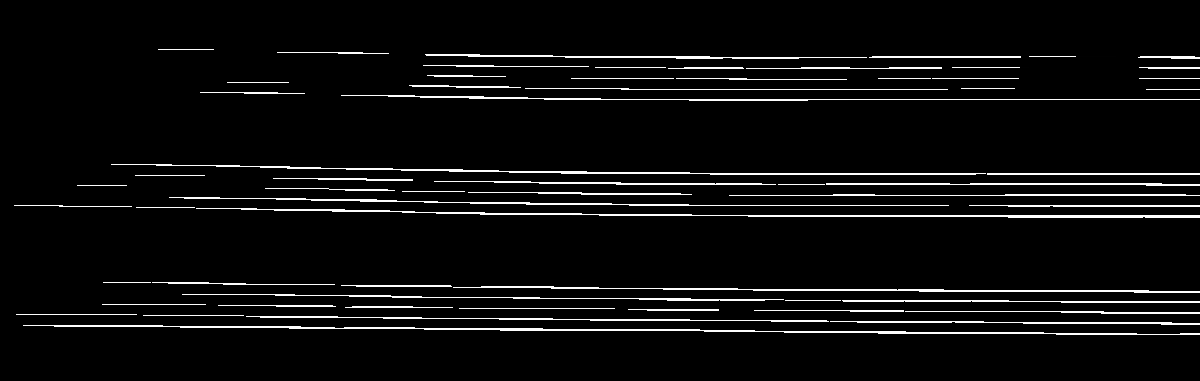
\includegraphics[width = \imagewidth]{4_horizontal_lines}
    \caption[Horizontal lines]{Wykryte linie poziome (do usunięcia)}
    \label{img:horizontal-lines}
    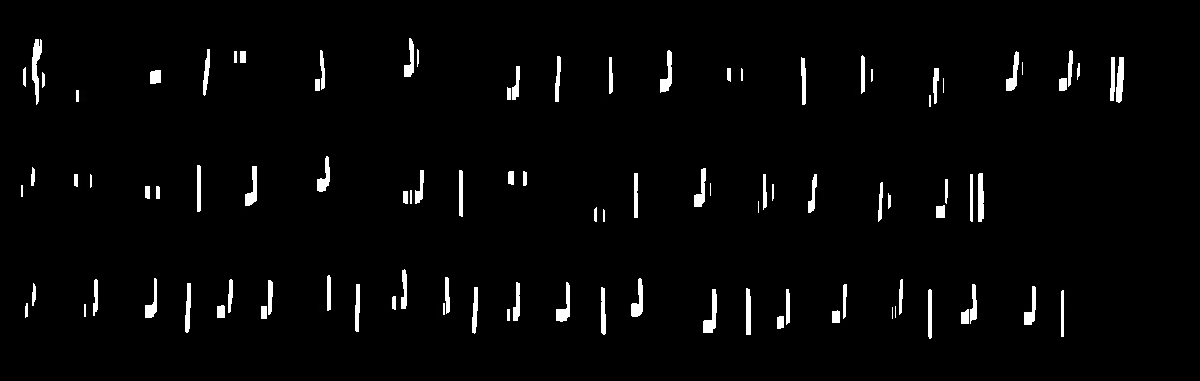
\includegraphics[width = \imagewidth]{5_vertical_lines}
    \caption[Horizontal lines]{Wykryte linie pionowe (do odbudowy)}
    \label{img:vertical-lines}
    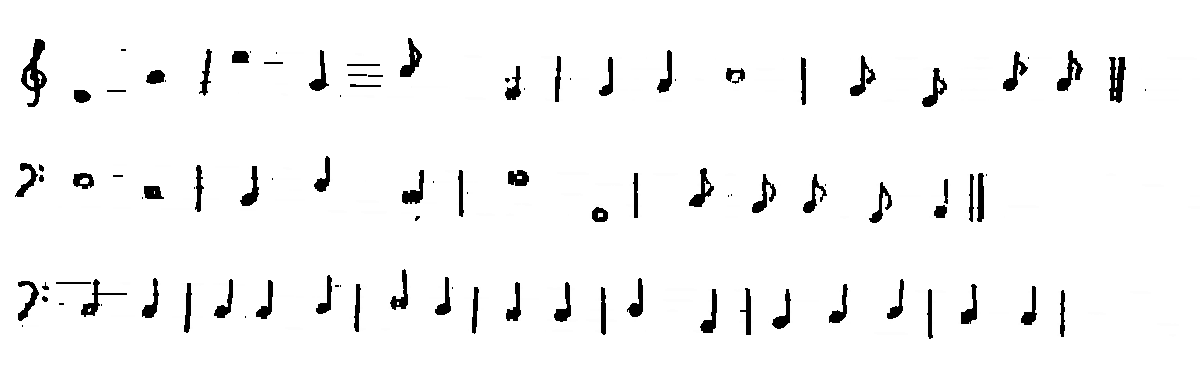
\includegraphics[width = \imagewidth]{6_erased}
    \caption[Horizontal lines]{Obraz z usuniętą pięciolinią}
    \label{img:removed-staff}
\end{figure}


\subsubsection{Usuwanie pięciolinii}
\label{subsec:staff-removal}
Wykryte w poprzednim podpunkcie linie poziome są usuwane z obrazu
z wykorzystaniem logicznego operatora OR.
\\
\\
W rezultacie pozostaje jednak wiele niewyeliminowanych, samotnych pikseli.
Piksele te usuwane usuwane są morfologiczną operacją domknięcia
z elementem strukturalnym o kształcie małego prostokąta.
\\
\\
Na końcu tego etapu następuje istotny punkt przetwarzania -
odbudowa uszkodzonych nut z użyciem otwarcia i wykrytych uprzednio linii pionowych.
\\
\\
Efekty usunięcia pięciolinii zostały przedstawione na
rysunku \ref{img:removed-staff}

\subsection{Object detection}
\label{sec:detection}
Po usunięciu pięciolinii następuje etap wyodrębniania symboli ze zdjęcia.
Wykorzystywany jest do tego sparametryzowany algorytm \emph{Connected-Components Labeling}
zaimplementowany w OpenCV.
Wykrywane są obiekty, których wielkość mieści się w ustalonym zakresie (rysunek \ref{img:detected-objects}).
\\
\\
Tej samej operacji poddawane są linie poziome (obraz źródłowy: rysunek \ref{img:horizontal-lines}),
które na tym etapie można już rozumieć jako linie wchodzące w skład pięciolinii.
Dodatkowo, ze względu na dość duże poszatkowanie obrazu źródłowego (rysunek \ref{img:detected-stafflines}),
algorytm uzupełnia brakujące linie interpolując wartości pochodzące ze
zbioru wszystkich wykrytych linii.

Algorytm rozdzielania pięciolinii jest oparty o odległość
między liniami - jeśli wykryta zostanie znacząca przestrzeń między liniami
to uznawana jest ona za granicę między pięcioliniami (rysunek \ref{img:detected-staves}).

\begin{figure}
    \centering
    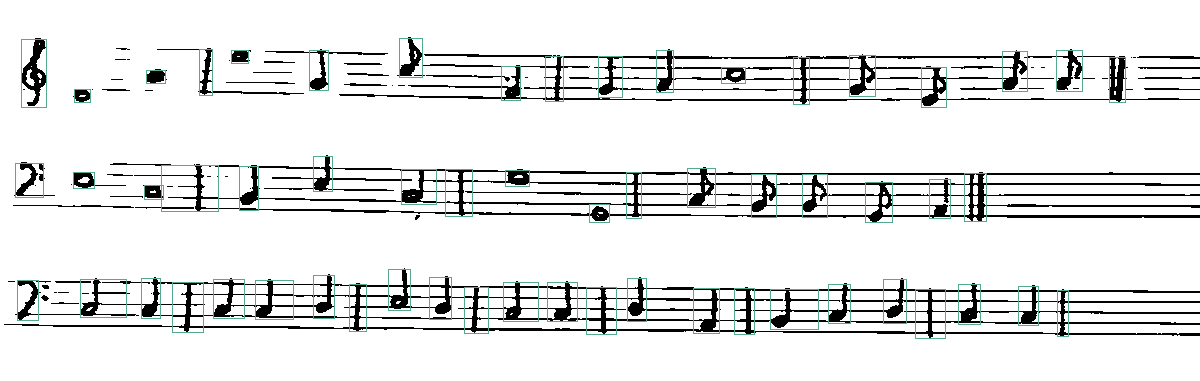
\includegraphics[width = \imagewidth]{7_detected_objects}
    \caption[Detected objects]{Wykryte obiekty (do klasyfikacji)}
    \label{img:detected-objects}
    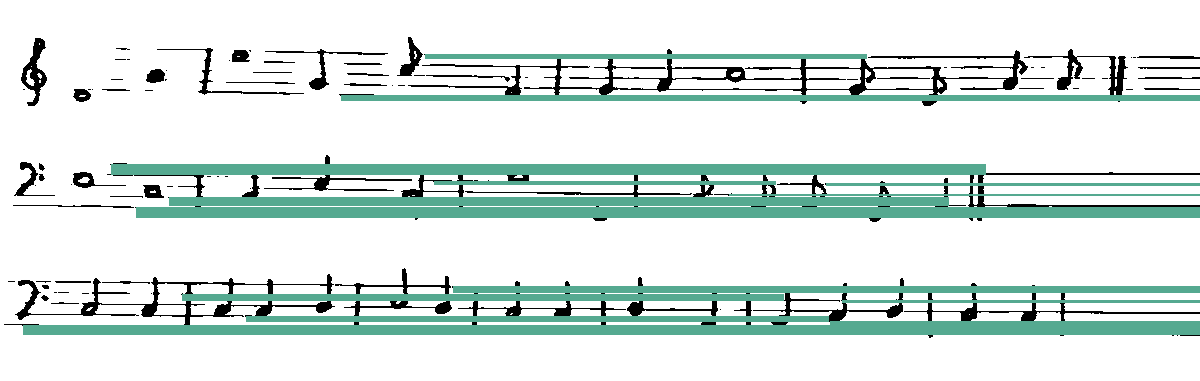
\includegraphics[width = \imagewidth]{8_detected_stafflines}
    \caption[Detected stafflines]{Wykryte linie pięciolinii}
    \label{img:detected-stafflines}
    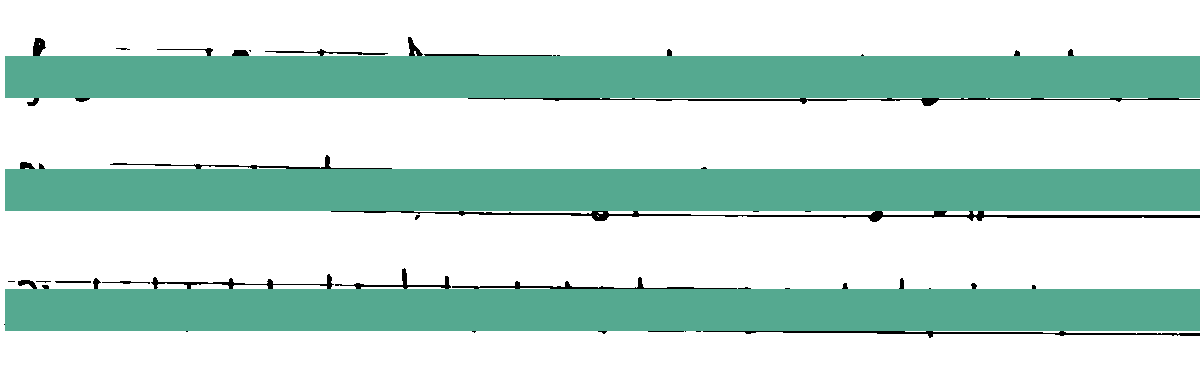
\includegraphics[width = \imagewidth]{9_detected_staves}
    \caption[Detected staves]{Wykryte pięciolinie}
    \label{img:detected-staves}
\end{figure}

\subsection{Object recognition}
\label{sec:recognition}

\subsubsection{Ograniczenia}
Na początku musimy zdefiniować kilka ograniczeń, na których będzie bazować
rozpoznawanie wykrytych obiektów.
\begin{itemize}
    \item Ograniczenia dziedzinowe
          \begin{itemize}
              \item Klucz wiolinowy (\clefG) jest zdecydowanie wyższy od wysokości pięciolinii
              \item Klucz basowy (\clefF) jest mniejszy niż wysokość pięciolinii.
              \item Główki nut mają wysokość jednego odstępu między liniami pięciolinii
          \end{itemize}

    \item Dodatkowe założenia
          \begin{itemize}
              \item Każda pięciolinia zawierająca nuty rozpoczyna się kluczem
              \item Główki nut mają horyzontalny aspect ratio (\geq 1:1): szerokość jest co najmniej równa wysokości
              \item Laseczki nut znajdują się zawsze nad główką, po prawej stronie.
          \end{itemize}
\end{itemize}


\subsubsection{Rozpoznawanie kluczy}
Rozpoznawanie kluczy oparto na naiwnym podejściu wykorzystującym
założenia podane powyżej:
\\\\
Wybieramy pierwsze obiekty z pięciolinii i bazując na założeniach
1 i 2 klasyfikujemy je na podstawie ich wysokości.

\subsubsection{Rozpoznawanie nut}
Rozpoznawanie rodzaju opiera się na charakterystycznej budowie nuty:
każda nuta składa się z główki (\textit{head}) i opcjonalnej laseczki (\textit{stem}).
W rozpatrywanych przypadkach mamy dwa rodzaje główek:
\begin{itemize}
    \item pełną (closed)
    \item otwartą (open)
\end{itemize}
oraz trzy rozpatrywane opcje laseczek:
\begin{itemize}
    \item brak laseczki
    \item pełną laseczkę (whole)
    \item laseczkę ósemkową (quaver)
\end{itemize}

Dzięki temu możemy określić minimalne charakterystyczne kombinacje tych elementów dla każdego rodzaju nut:

\begin{description}
    \item [cała nuta (\textit{semibreve})] - nie posiada laseczki
    \item [półnuta (\textit{minim})] - posiada pełną laseczkę oraz otwartą główkę
    \item [ćwierćnuta (\textit{crotchet})] - posiada pełną laseczkę i pełną główkę
    \item [ósemka (\textit{quaver})] - posiada ósemkową laseczkę
\end{description}

\paragraph*{Rozpoznawanie laseczki}
Algorytm rozpoznawania laseczki bazuje na analizie sum kolumn i rzędów obrazu.
Przebiega on według następującego schematu:
\begin{enumerate}
    \item Mając dany czarno-biały obraz nuty zaneguj go tak, aby nuta miała kolor biały (`negatyw`).
    \item Znormalizuj negatyw do postaci zmiennoprzecinkowej z zakresu 0.0 - 1.0.
    \item Stwórz wektor sum kolumnowych (`kolumny`) po wszystkich kolumnach negatywu.
    \item Ustal próg definiujący minimalną wysokość głównej laseczki (`próg`).
    \item Przefiltruj stabilnie kolumny eliminując te, które nie przekraczają progu.
    \item Z pozostałych kolumn wybierz tę z najniższym indeksem - będzie to lewa granica laseczki (`left offset`).
    \item Jeśli nie istnieje taka kolumna, to \textbf{nuta nie posiada laseczki}.
    \item Ogranicz negatyw od lewej strony przez left offset.
    \item Ustal próg definiujący minimalną wysokość ósemkowej laseczki (`próg ósemkowy`).
    \item Przefiltruj stabilnie kolumny eliminując te, które nie przekraczają progu ósemkowego.
    \item Z pozostałych kolumn wybierz tę z najniższym indeksem - będzie to lewa granica laseczki (`right offset`).
    \item Analogicznie postępuj dla rzędów, aby ograniczyć laseczkę od góry i od dołu.
    \item Wybierz najwęższy  i najszerszy odcinek laseczki.
    \item Jeśli najszerszy odcinek jest przynajmniej trzykrotnie większy niż najwęższy odcinek, to uznajemy laseczkę za ósemkową, w przeciwnym przypadku uznajemy laseczkę za pełną.
\end{enumerate}

\paragraph*{Rozpoznawanie główki}
Algorytm rozpoznający główkę działa analogicznie do algorytmu
rozpoznającego laseczkę. Najpierw odcinamy z obrazu część z laseczką,
następnie tworzymy negatyw i znajdujemy lewy, prawy, górny i dolny offset.
\\\\
Typ główki rozpoznajemy na podstawie punktu centralnego główki:
wyznaczamy środek główki, obliczamy sumę w środkowym rzędzie
oraz środkowej kolumnie. Uznajemy, że główka jest pełna,
jeśli obie sumy są większe od, odpowiednio, połowy długości i
połowy szerokości główki.

\part*{Przykłady}


\end{document}